\documentclass[11pt,a4paper]{article}
\usepackage[T1]{fontenc}
\usepackage[utf8]{inputenc}
\usepackage{lmodern}
\usepackage[margin=2.6cm]{geometry}
\usepackage{amsmath,amssymb}
\usepackage{graphicx}
\usepackage{booktabs,longtable,array}
\usepackage[round,authoryear]{natbib}
\usepackage[hidelinks]{hyperref}
\usepackage{xcolor}
\usepackage{caption}
\captionsetup{font=small,labelfont=bf}
\setlength{\parskip}{0.45em}
\setlength{\parindent}{0pt}
\graphicspath{{../figures/}}
% generated by paper/make_numbers.py -- do not edit by hand
\newcommand{\AmpBaseB}{4.24}
\newcommand{\AmpCorr}{0.43}
\newcommand{\AmpCtrlB}{3.13}
\newcommand{\AmpCtrlP}{$p<0.001$}
\newcommand{\AmpGammaB}{1.75}
\newcommand{\AmpN}{42}
\newcommand{\AmpShare}{26}
\newcommand{\AmpShareK}{18}
\newcommand{\AmpShareNoRus}{26}
\newcommand{\CatchBetaMax}{0.84}
\newcommand{\CatchBetaMin}{0.69}
\newcommand{\CatchLooMin}{0.58}
\newcommand{\CatchPMax}{0.004}
\newcommand{\ConvBetaMax}{0.70}
\newcommand{\ConvBetaMin}{0.53}
\newcommand{\ConvPMax}{0.086}
\newcommand{\ConvPMin}{0.049}
\newcommand{\DeepDomIcioP}{0.025}
\newcommand{\DeepDomWiodP}{0.468}
\newcommand{\DeepIcioP}{0.52}
\newcommand{\DeepWiodP}{0.12}
\newcommand{\DomIcioBeta}{0.16}
\newcommand{\DomIcioP}{$p=0.770$}
\newcommand{\DomWiodBetaMax}{0.50}
\newcommand{\DomWiodBetaMin}{0.42}
\newcommand{\DomWiodPMax}{0.075}
\newcommand{\DomWiodPMin}{0.037}
\newcommand{\FcConstRmse}{2.41}
\newcommand{\FcCorr}{0.64}
\newcommand{\FcN}{42}
\newcommand{\FcPastCorr}{0.62}
\newcommand{\FcPastRmse}{2.46}
\newcommand{\FcRmse}{2.19}
\newcommand{\FcSameCorr}{0.55}
\newcommand{\FcSameRmse}{2.21}
\newcommand{\FinalPartB}{0.41}
\newcommand{\FinalPartP}{0.41}
\newcommand{\ImpIcioHourPMax}{0.16}
\newcommand{\ImpIcioHourPMin}{0.12}
\newcommand{\ImpIcioPcPMax}{0.61}
\newcommand{\ImpIcioPcPMin}{0.58}
\newcommand{\ImpWiodPMax}{0.005}
\newcommand{\ModelRsq}{0.85}
\newcommand{\ModelSlope}{1.08}
\newcommand{\NEstimates}{55}
\newcommand{\NIcio}{30}
\newcommand{\NWiod}{43}
\newcommand{\NetPartB}{1.48}
\newcommand{\NetPartP}{$p=0.011$}
\newcommand{\PooledIcioBeta}{0.88}
\newcommand{\PooledIcioP}{$p=0.012$}
\newcommand{\PooledWiodBeta}{0.81}
\newcommand{\PooledWiodP}{$p=0.002$}
\newcommand{\PriceBeta}{$-0.26$}
\newcommand{\PriceDomBeta}{$-0.15$}
\newcommand{\PriceDomIndP}{0.93}
\newcommand{\PriceDomP}{$p=0.041$}
\newcommand{\PriceIndBeta}{$-0.05$}
\newcommand{\PriceIndP}{0.70}
\newcommand{\PriceN}{2{,}224}
\newcommand{\PriceP}{$p<0.001$}
\newcommand{\RankAustraliaDom}{5}
\newcommand{\RankAustraliaFar}{15}
\newcommand{\RankCorr}{0.45}
\newcommand{\RankIrelandDom}{30}
\newcommand{\RankIrelandFar}{22}
\newcommand{\RankLuxembourgDom}{27}
\newcommand{\RankLuxembourgFar}{2}
\newcommand{\RankUsaDom}{14}
\newcommand{\RankUsaFar}{29}
\newcommand{\RawRMax}{0.66}
\newcommand{\RawRMin}{0.63}
\newcommand{\SpearWeights}{0.98}
\newcommand{\WithinIcioP}{0.81}
\newcommand{\WithinWiodP}{0.24}


\newcommand{\Lbar}{\bar L}

\title{\textbf{Do Longer Production Chains Make Economies Grow Faster?}\\[0.3em]
\large An independent replication and stress test of the production-network\\amplification hypothesis}
\author{Stefano Restelli\\
\small Independent researcher, Berlin\\
\small \href{mailto:stefano.restelli15@gmail.com}{stefano.restelli15@gmail.com}}
\date{\small Working paper, November 2026 --- draft v0.1\\
Code and data: \url{https://github.com/therestofeden/illuminations}}

\begin{document}
\maketitle

\begin{abstract}
\noindent
\citet{mcnerney2022} argue that economies with longer production chains grow
faster, because each improvement in an upstream industry is passed down, and
compounded, along every chain that uses its output. We replicate and stress-test
this claim on two independent input--output databases (WIOD 2016, \NWiod{}
economies, 2000--2014; OECD ICIO 2023, \NIcio{} economies, 2011--2020), with
growth of real GDP per hour from the Penn World Table 11.0, over horizons up to
2023. Four findings. (i) Measurement matters: cutting chains at the national
border, a common shortcut, reshuffles country rankings (rank correlation
\RankCorr{}) and hides most of the effect. (ii) With the paper's own
definition, the cross-country pattern replicates in both databases and every
horizon: one standard deviation of chain length goes with
\CatchBetaMin{}--\CatchBetaMax{} percentage points a year of faster
productivity growth after controlling for catch-up ($p\le\CatchPMax$,
permutation tests). It survives dropping China, Vietnam and the post-2004 EU
members, though only marginally, and survives a control for reliance on imported
inputs in one database but not the other. (iii) About \AmpShare\% of the
cross-country slope is composition (long-chain economies also contain
faster-improving industries); the rest behaves as the amplification story
predicts, and a zero-parameter forecast built on it beats simpler benchmarks,
modestly. (iv) The pattern is a \emph{between}-country regularity: we find no
detectable effect of a country's own chains lengthening on its subsequent
growth, and the price mechanism holds across industry types but not for the same
industry in different countries. The production-network view survives as a
robust cross-country fact; its causal reading remains open.
\end{abstract}

\section{What are we trying to understand?}\label{sec:intro}

Bread does not come from a bakery alone. A farm grows wheat, a mill turns it into
flour, a bakery turns flour into bread, and each of those firms buys machines,
energy, transport and services from yet other firms. Every product sits at the end
of a web of such chains. Some chains are short: a farmer selling vegetables at a
market uses little besides her own work and land. Others are long: a car is the
last link of chains that run through steel, glass, chips, software and logistics.

Ecologists have a word for the position of a species in a food web: its
\emph{trophic level}. Plants are at level one, herbivores at two, predators that
eat herbivores at three \citep{levine1980}. The same arithmetic applies to an
economy's input--output table, and it produces a number for every industry: how
many production steps, on average, stand behind one euro of its output.

Why should anyone care how long the chains are? Because improvements travel
along them. Suppose each firm in the wheat--flour--bread chain becomes 1\% more
efficient this year, in the sense that it needs 1\% fewer inputs per unit of
output. Wheat becomes about 1\% cheaper relative to wages. Flour benefits
twice: from the mill's own improvement and from cheaper wheat. Bread benefits
three times. The longer the chain, the more improvements compound into the price
of the final good, and the more a worker's wage can buy. This is the core of the
argument made by \citet{mcnerney2022} and popularised in \citet{farmer2024}:
\emph{production networks amplify technological progress, so economies whose
spending runs through longer chains should grow faster}.

The claim matters for at least three reasons. It offers a structural explanation
for why some countries grow faster than others, beyond capital accumulation and
education. It bears on industrial policy: if chain length amplifies growth,
policies that ``deepen'' a domestic industrial base, or plug a country into
global supply chains, could have payoffs beyond the industries they target. And
it connects economics to the broader science of complex networks, where the
position of a node in a directed network often determines how shocks propagate
through it \citep{acemoglu2012,mackay2020}.

The original paper supports the claim with data from the World Input--Output
Database for 1995--2009, finding a correlation of 0.53 between countries' average
chain length and their subsequent growth. A single correlation on one dataset and
one period is a reasonable start, but it leaves open the questions a careful reader
would ask next:

\begin{enumerate}
\item \textbf{Does it replicate?} On a different database, in a later period, with
the paper's own outcome (growth of output per hour worked)?
\item \textbf{Is it chains, or something that travels with them?} Countries with
long chains are often fast-converging manufacturing economies (China, Central
Europe), deeply integrated in global supply chains. Is chain length doing the
work, or catch-up, or trade integration?
\item \textbf{Is it the multiplication or the ingredients?} The model says growth
is roughly \emph{chain length times the speed at which industries improve}. Long
chains could matter because they multiply improvements (amplification), or simply
because long-chain economies happen to contain faster-improving industries
(composition).
\item \textbf{Does it work within a country?} If a country's chains lengthen, does
it subsequently grow faster? And do prices actually fall faster at the end of
long chains, as the mechanism requires?
\end{enumerate}

This paper answers each question with public data and openly available code. We
report every specification we ran (\NEstimates{} estimates in the main grid, plus
the amplification tests), and use resampling-based inference, since the samples
are small ($30$--$43$ countries).

\paragraph{Preview of results.} The cross-country pattern is real and robust;
how one measures chain length matters a great deal; about a quarter of the
pattern is composition; and nothing in our data shows the effect operating
within countries over time. Section~\ref{sec:discussion} discusses what this does
and does not imply.

\section{The idea in one equation}\label{sec:theory}

Let $Z_{ij}$ be the value of goods industry $i$ sells to industry $j$ in a year,
$x_j$ the gross output of $j$, and $A_{ij}=Z_{ij}/x_j$ the input coefficient: how
many euros of $i$ go into one euro of $j$. The \emph{output multiplier} of
industry $j$ is defined recursively as
\begin{equation}
L_j \;=\; 1 + \sum_i A_{ij} L_i
\qquad\Longleftrightarrow\qquad
L = (I - A^\top)^{-1}\mathbf{1}. \label{eq:L}
\end{equation}
An industry that buys only labour and capital has $L=1$. An industry that spends
half of its revenue on inputs from industries with $L=2$ has $L=2$. In this sense
$L_j$ counts the average number of production stages behind industry $j$: it is
the trophic level of the industry. It coincides with the ``production
staging'' measure of \citet{fally2012} and the input downstreamness of
\citet{miller2017}, and is the mirror image of the upstreamness (distance to
final use) of \citet{antras2012}.

A country's \textbf{average chain length} weights its industries by their share
$\theta_i$ of final demand (household consumption, government, investment),
\begin{equation}
\Lbar_c = \sum_{i\in c}\theta_i L_i,\qquad \theta_i = \frac{y_i}{\sum_{j\in c}y_j},
\label{eq:Lbar}
\end{equation}
where $L$ is computed on the \emph{world} input--output table, so a chain counts
the steps performed abroad as well \citep[eq.~5]{mcnerney2022}. In a closed
economy, $\Lbar$ equals gross output divided by GDP: how many euros of sales
change hands for each euro of final value created.

\paragraph{The prediction.} Let $\gamma_i$ be the rate at which industry $i$
reduces the inputs it needs per unit of output (its productivity growth). With
competitive pricing, prices relative to wages change at
$r=-(I-A^\top)^{-1}\gamma$, so the growth in what a unit of labour can buy is
\begin{equation}
g \;=\; \theta^\top (I-A^\top)^{-1}\gamma
\;\;\overset{\gamma_i=\bar\gamma}{=}\;\; \bar\gamma\,\Lbar .
\label{eq:g}
\end{equation}
If all industries improved at the same rate, growth would be exactly
proportional to chain length. More generally, in a closed economy
$g=\Lbar\,\tilde\gamma$, where $\tilde\gamma$ is the gross-output-weighted
average of $\gamma_i$: this is Hulten's theorem \citep{domar1961,hulten1978}.

\paragraph{What is accounting and what is a claim about the world.}
Equation~\eqref{eq:g} is close to an identity: \emph{given} industry productivity
growth, chain length must matter. The empirical content of the hypothesis is
elsewhere. It is that (a) countries differ enough in $\Lbar$, persistently enough,
for chain length to predict growth \emph{ahead}; and (b) the differences in
$\Lbar$ are not offset by long-chain economies having slower-improving industries
(or, conversely, that the link is not merely because they have faster ones). Our
tests are designed around these two points rather than around the identity.

\section{Related literature}\label{sec:lit}

Three literatures meet here. The first measures the position of industries along
production chains: production staging \citep{fally2012}, upstreamness and
downstreamness \citep{antras2012,miller2017}, and decompositions of production
length within and across borders \citep{wang2017}. These papers document
patterns; \citet{mcnerney2022} add a growth mechanism.

The second studies how industry-level productivity aggregates through production
networks: from \citet{domar1961} and \citet{hulten1978} to the network origins of
aggregate fluctuations \citep{acemoglu2012} and the non-linear corrections of
\citet{baqaee2019}. The role of intermediate inputs as multipliers in
development is emphasised by \citet{ciccone2002} and \citet{jones2011}.

The third comes from complexity science: measures of economic complexity
\citep{hidalgo2009} and of trophic coherence in directed networks
\citep{mackay2020} treat the economy's structure as informative about its
capabilities. \citet{farmer2024} brings these strands together for a general
audience. This paper contributes an independent, transparent test of the growth
claim, rather than a new measure or model.

\section{Data}\label{sec:data}

\begin{itemize}
\item \textbf{WIOD 2016 release} \citep{timmer2015,wiod2016}: world input--output
tables for \NWiod{} economies plus a rest-of-world region, 56 industries,
2000--2014, with Socio-Economic Accounts (prices, volumes, labour and capital
compensation) used for productivity growth and price tests. This is the database
family used by \citet{mcnerney2022}.
\item \textbf{OECD ICIO, 2023 edition} \citep{oecdicio2023}: 76 economies and 45
industries; we use the \NIcio{} economies of our original study for 2011--2020.
\item \textbf{Penn World Table 11.0} \citep{feenstra2015,pwt110}: real GDP at
constant national prices (\texttt{rgdpna}) for growth, persons engaged times
average hours for labour input, and output-side real GDP at PPPs
(\texttt{rgdpo}) for comparisons of productivity \emph{levels} across countries.
\end{itemize}

All sources are free to reuse with attribution (CC BY 4.0 for WIOD and PWT; OECD
terms of use). The raw tables are downloaded by scripts in the repository.

\section{Methods}\label{sec:methods}

\paragraph{Measures.} For every year and database we compute: Farmer's chain
length $\Lbar_c$ (equation~\ref{eq:Lbar}); a \emph{domestic} variant that solves
equation~\eqref{eq:L} on the country's own block of the table, treating imported
inputs like labour, and weights by gross output (the definition used in an
earlier version of our own study); gross output over value added; and
\emph{import intensity}, imported intermediates over gross output.

\paragraph{Outcomes and controls.} Growth is the average annual log change of
real GDP per hour worked. Every growth regression controls for the initial
level of GDP per hour at PPP, because poorer economies grow faster for reasons
unrelated to chains \citep{barro1991}.

\paragraph{Specifications.} (A) cross-sections, depth at the start of a window
against growth over it: ICIO 2011$\to$2019 and 2011$\to$2023; WIOD
2000$\to$2014, 2019 and 2023; (B) pooled non-overlapping windows with period
effects, and the same with country fixed effects (within-country); (C) a
``deepening'' test: change in depth over the previous three years against growth
over the next three, with and without lagged growth; (D) a price test across
\PriceN{} industries: annual change of each industry's output price relative to
the economy-wide wage, 2000--2014, against its 2000 multiplier, with country
fixed effects and then also with industry fixed effects.

\paragraph{Productivity growth.} For the amplification tests we compute
gross-output productivity growth for every WIOD industry,
$\gamma_i=\Delta\ln Q_i - s^{M}_i\,\Delta\ln M_i - s^{L}_i\,\Delta\ln N_i$, from
real output $Q$, real intermediate inputs $M$ and persons engaged $N$, with
average cost shares $s$; a variant also nets out capital. Industries with missing
data (and the rest-of-world region) take the output-weighted cross-country mean
of the same industry; Russia has \textasciitilde{}41\% of industries imputed, so
every test is also run without it.

\paragraph{Inference.} With 30--43 countries, analytic standard errors can
mislead. For cross-sections we report Freedman--Lane permutation $p$-values
\citep{freedman1983}; for panels, wild-cluster bootstrap $p$-values with
Rademacher weights, clustered by country \citep{cameron2008}; 4,999 draws, fixed
seed. We report every specification in the grid, in the spirit of specification
curve analysis \citep{simonsohn2020}; Appendix~\ref{app:all} lists all of them.

\section{Results}\label{sec:results}

\subsection{How you measure chain length changes who is ``deep''}

Figure~\ref{fig:rerank} ranks the \NIcio{} ICIO economies in 2019 by the domestic
measure and by Farmer's measure. The weights barely matter (rank correlation
\SpearWeights{} between output and final-demand weights); the border matters a
lot (\RankCorr{}). Luxembourg moves from \RankLuxembourgDom{}th to
\RankLuxembourgFar{}nd, Ireland from \RankIrelandDom{}th to \RankIrelandFar{}nd,
the United States from \RankUsaDom{}th to \RankUsaFar{}th. Small open economies
assemble goods whose earlier stages happen abroad; a domestic measure sees a
short chain, the world table sees a long one. For the amplification mechanism the
world table is the relevant one: a Vietnamese phone gets cheaper when Korean chip
makers improve.

\begin{figure}[t]
\centering
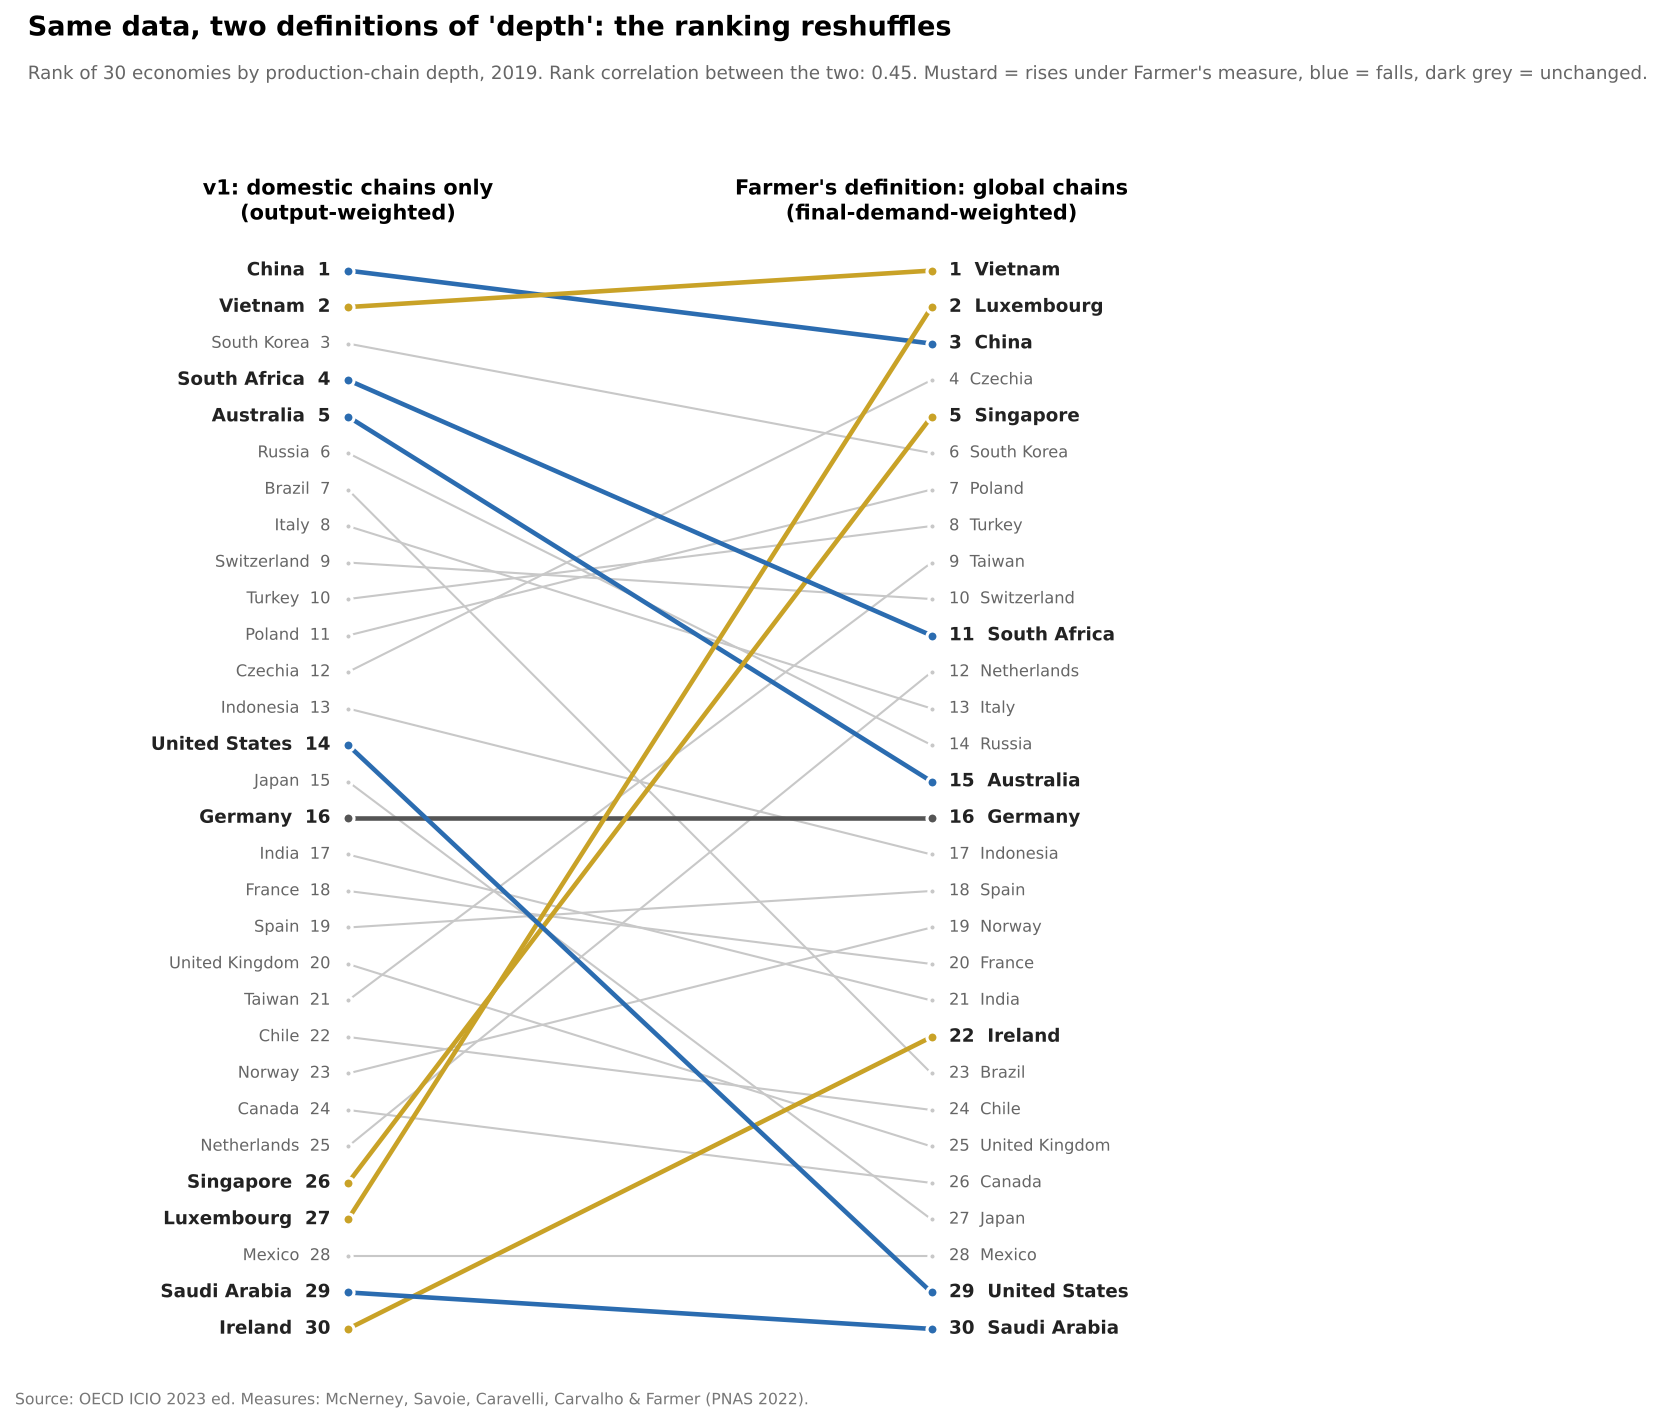
\includegraphics[width=0.72\textwidth]{9_measure_rerank.png}
\caption{Ranking of 30 economies by chain length in 2019: domestic chains only
(left) versus Farmer's global, final-demand-weighted measure (right).}
\label{fig:rerank}
\end{figure}

\subsection{The cross-country pattern replicates}

Table~\ref{tab:main} and Figure~\ref{fig:replication} show the central result.
With Farmer's measure, chain length at the start of a window predicts growth of
GDP per hour over it in both databases and at every horizon. The raw
correlations are \RawRMin{}--\RawRMax{} (the original paper reports 0.53 for
1995--2009). After the catch-up control, one standard deviation of chain length
goes with \CatchBetaMin{}--\CatchBetaMax{} percentage points a year of extra
growth, all with $p\le\CatchPMax$; dropping any single country never pushes the
estimate below \CatchLooMin{}. The domestic measure gives much weaker results:
\DomIcioBeta{} on ICIO (\DomIcioP) and \DomWiodBetaMin{}--\DomWiodBetaMax{} on WIOD
($p$ between \DomWiodPMin{} and \DomWiodPMax{}).

\begin{table}[t]
\centering
\caption{Chain length at the start of the window and growth of GDP per hour over
it. Coefficients per standard deviation of the depth measure, in percentage
points a year, controlling for the initial PPP level of GDP per hour.
Permutation $p$-values (4,999 draws).}
\label{tab:main}
\begin{tabular}{lrrrrr}
\toprule
 & \multicolumn{2}{c}{Farmer's $\bar L$ (global)} & \multicolumn{2}{c}{Domestic depth (v1)} & \\
\cmidrule(lr){2-3}\cmidrule(lr){4-5}
Sample & $\beta$/SD & $p$ & $\beta$/SD & $p$ & $n$ \\
\midrule
ICIO, 2011--2019 & +0.84 & 0.004 & +0.16 & 0.770 & 30 \\
ICIO, 2011--2023 & +0.83 & 0.003 & +0.29 & 0.592 & 30 \\
WIOD, 2000--2014 & +0.70 & $<0.001$ & +0.50 & 0.037 & 42 \\
WIOD, 2000--2019 & +0.69 & $<0.001$ & +0.47 & 0.048 & 43 \\
WIOD, 2000--2023 & +0.69 & $<0.001$ & +0.42 & 0.075 & 43 \\
\bottomrule
\end{tabular}

\end{table}

\begin{figure}[t]
\centering
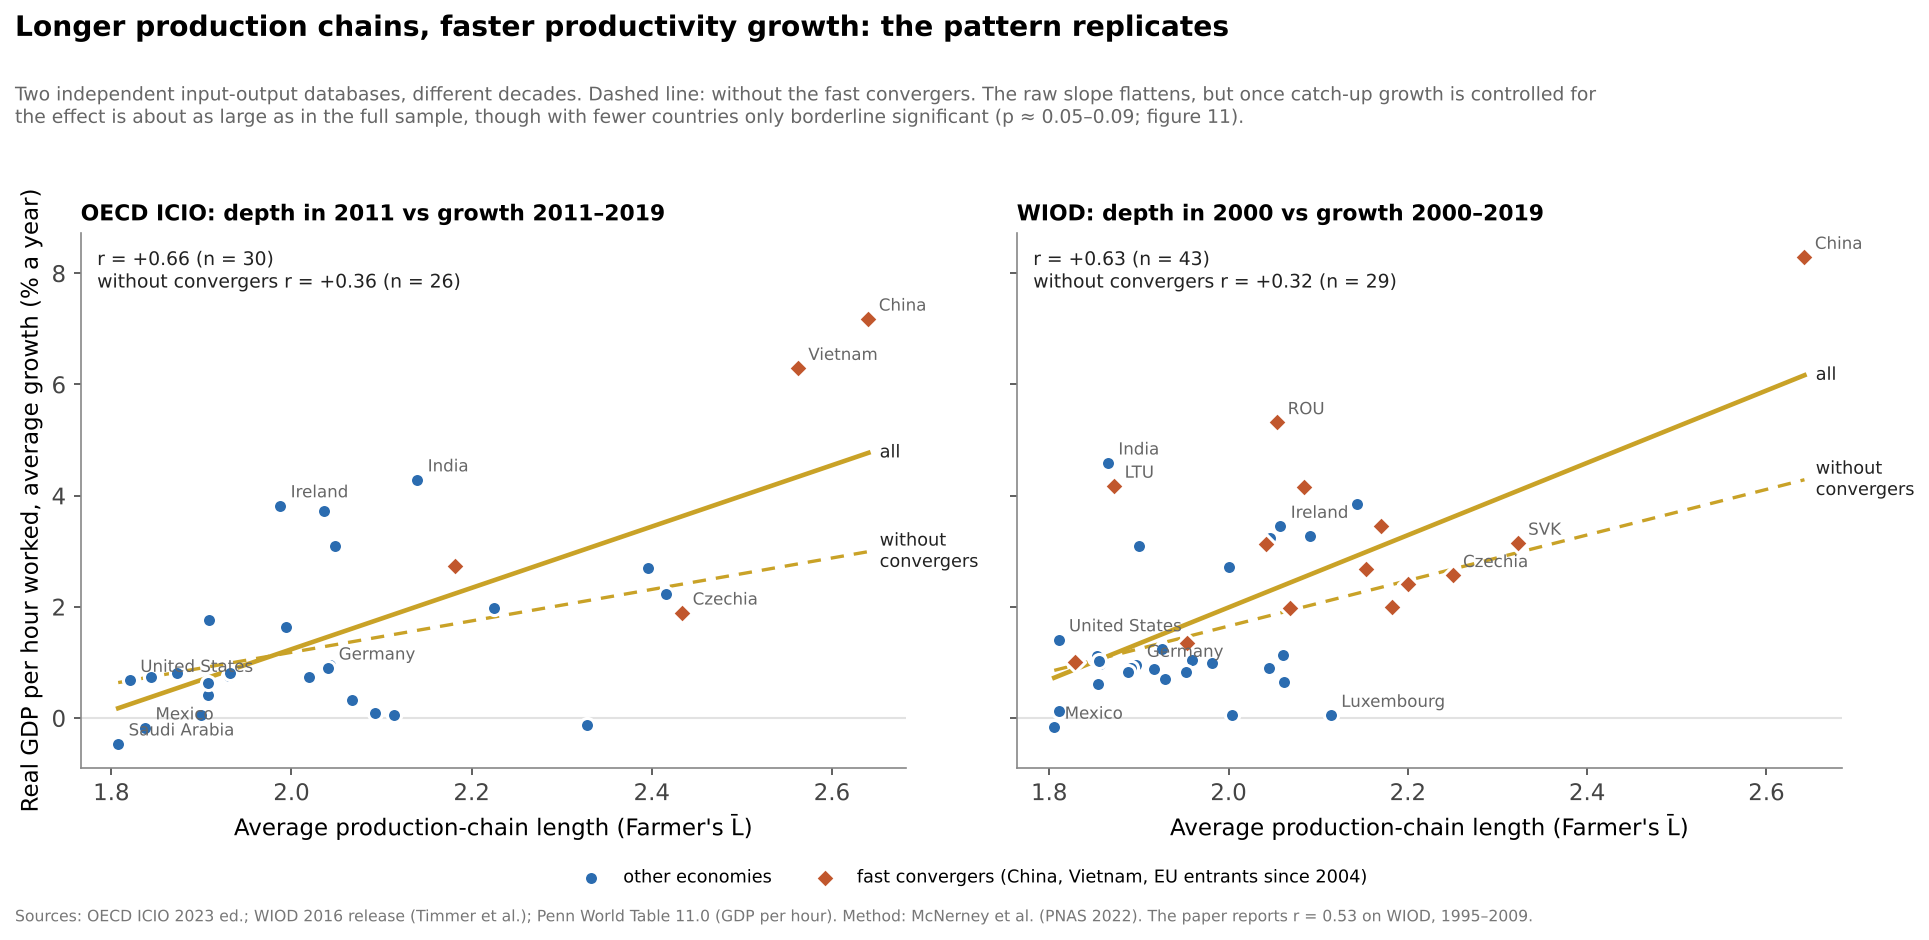
\includegraphics[width=\textwidth]{10_replication.png}
\caption{Chain length and later productivity growth in two independent databases.
Diamonds: China, Vietnam and EU members since 2004. Raw (uncontrolled) relations.}
\label{fig:replication}
\end{figure}

\subsection{Stress tests: convergers and supply-chain integration}

Two confounders are natural. First, the fast convergers: China, Vietnam and the
Central and Eastern European members of the EU. Accession and foreign investment
lengthened their chains \emph{and} raised their productivity at the same time.
Dropping them leaves estimates of \ConvBetaMin{}--\ConvBetaMax{}, close to the
full-sample values, with $p$ between \ConvPMin{} and \ConvPMax{}: the effect is
not driven by them, but with 26--29 countries left it is only marginally
significant. Second, integration in global supply chains: Farmer's measure rises
mechanically with imported inputs. Controlling for import intensity, the WIOD
results hold ($p\le\ImpWiodPMax$), while the ICIO results do not ($p$ between
\ImpIcioHourPMin{} and \ImpIcioPcPMax{}). With 30 countries we cannot separate
long chains from participation in global value chains in that sample.
Figure~\ref{fig:hold} puts all tests on one scale.

\begin{figure}[t]
\centering
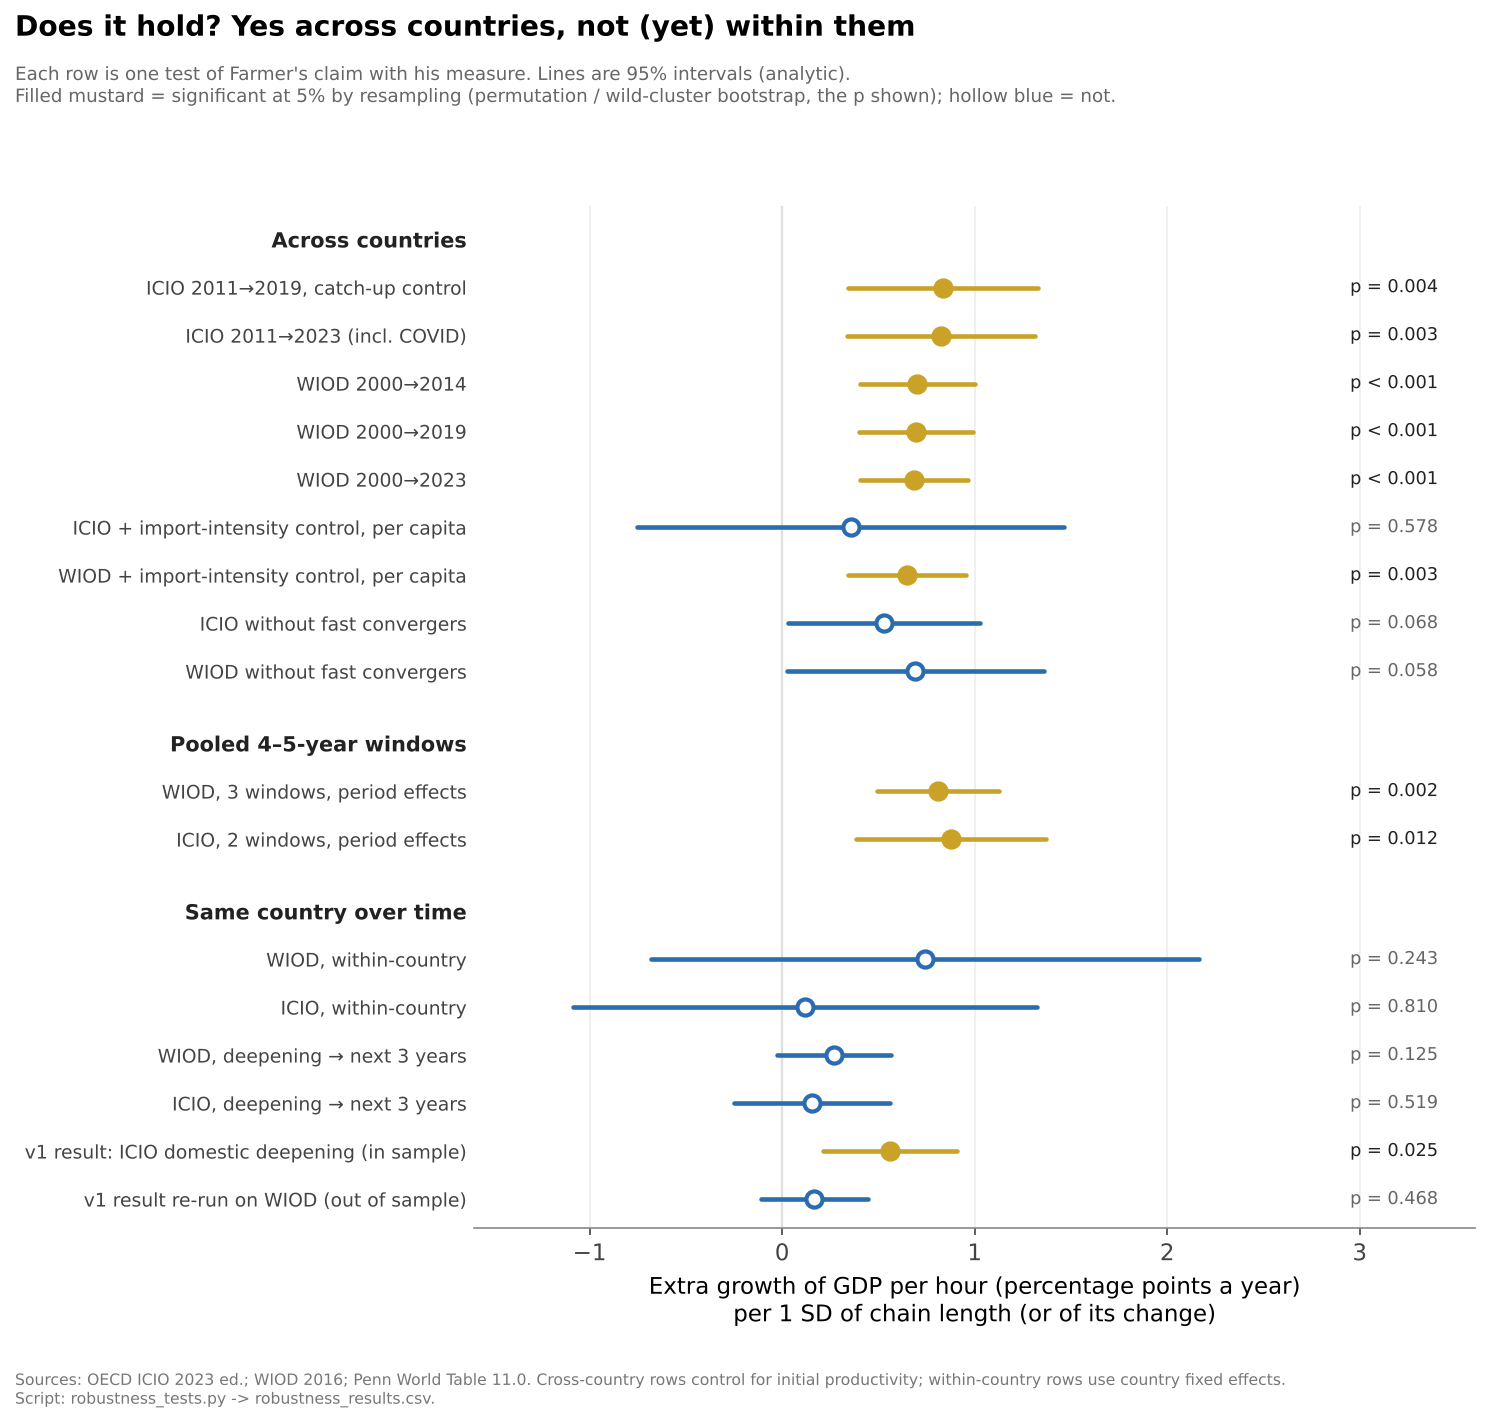
\includegraphics[width=0.85\textwidth]{11_does_it_hold.png}
\caption{Every test of the growth claim with Farmer's measure. Points are
estimates per standard deviation; lines are 95\% analytic intervals; filled
points are significant at 5\% by resampling.}
\label{fig:hold}
\end{figure}

\subsection{Chains or the industries in them?}

Table~\ref{tab:amp} turns to the full prediction, using industry productivity
growth $\gamma$ from WIOD for 2000--2014 (\AmpN{} economies). Long-chain economies
did contain faster-improving industries: the correlation between $\Lbar$ and
$\tilde\gamma$ is \AmpCorr{}. Holding $\tilde\gamma$ fixed reduces the
coefficient on chain length from \AmpBaseB{} to \AmpCtrlB{} (\AmpCtrlP): about
\AmpShare\% of the cross-country slope is composition, and the rest remains
(\AmpShareNoRus\% without Russia; \AmpShareK\% with $\gamma$ net of capital).
The model's full prediction, $\theta^\top(I-A^\top)^{-1}\gamma$, explains growth
with a slope of \ModelSlope{} ($R^2=\ModelRsq$ with the catch-up control), and
when it is split in two, the information sits in the network part (upstream
improvements, \NetPartB{}, \NetPartP) rather than in the final-stage industries'
own improvements (\FinalPartB{}, $p=\FinalPartP$). As Section~\ref{sec:theory}
warned, these last two results are close to accounting identities and are best
read as a consistency check of the framework, not as independent evidence.

\begin{table}[t]
\centering
\caption{Amplification versus composition, WIOD, growth of GDP per hour
2000--2014. All regressions include the catch-up control.}
\label{tab:amp}
\begin{tabular}{llrrr}
\toprule
Specification & Coefficient & Estimate & $p$ (perm.) & $R^2$ \\
\midrule
(1) chain length & $\bar L$ & +4.24 & $<0.001$ & 0.75 \\
(2) $+$ industry productivity $\tilde\gamma$ & $\bar L$ & +3.13 & $<0.001$ & 0.88 \\
 & $\tilde\gamma$ & +1.75 & $<0.001$ &  \\
(3) full model prediction & $\theta'(I-A^\top)^{-1}\gamma$ & +1.08 & $<0.001$ & 0.85 \\
(4) final-stage $+$ network part & final-stage part $\theta'\gamma$ & +0.41 & 0.413 & 0.86 \\
 & network part & +1.48 & 0.011 &  \\
\bottomrule
\end{tabular}

\end{table}

The test that is \emph{not} an identity is forecasting (Table~\ref{tab:fc},
Figure~\ref{fig:chains}, right). Using only information available in 2007,
chain length times past industry productivity growth predicts 2007--2014 growth
with a correlation of \FcCorr{}, against \FcSameCorr{} for the same forecast
without cross-country differences in chain length and \FcPastCorr{} for
``past growth continues''. The gain is real but modest, and the period includes
the global financial crisis.

\begin{table}[t]
\centering
\caption{Zero-parameter forecasts of mean growth of GDP per hour, 2007--2014,
from information available in 2007 (\FcN{} economies).}
\label{tab:fc}
\begin{tabular}{lrr}
\toprule
Forecast of 2007--2014 growth & Correlation & RMSE \\
\midrule
Farmer: $\bar L_{2007}\times\tilde\gamma_{2000\text{--}07}$ & 0.64 & 2.19 \\
Same $\tilde\gamma$, average chain length & 0.55 & 2.21 \\
Past growth continues (2000--07) & 0.62 & 2.46 \\
Everyone grows at the 2000--07 mean & -- & 2.41 \\
\bottomrule
\end{tabular}

\end{table}

\begin{figure}[t]
\centering
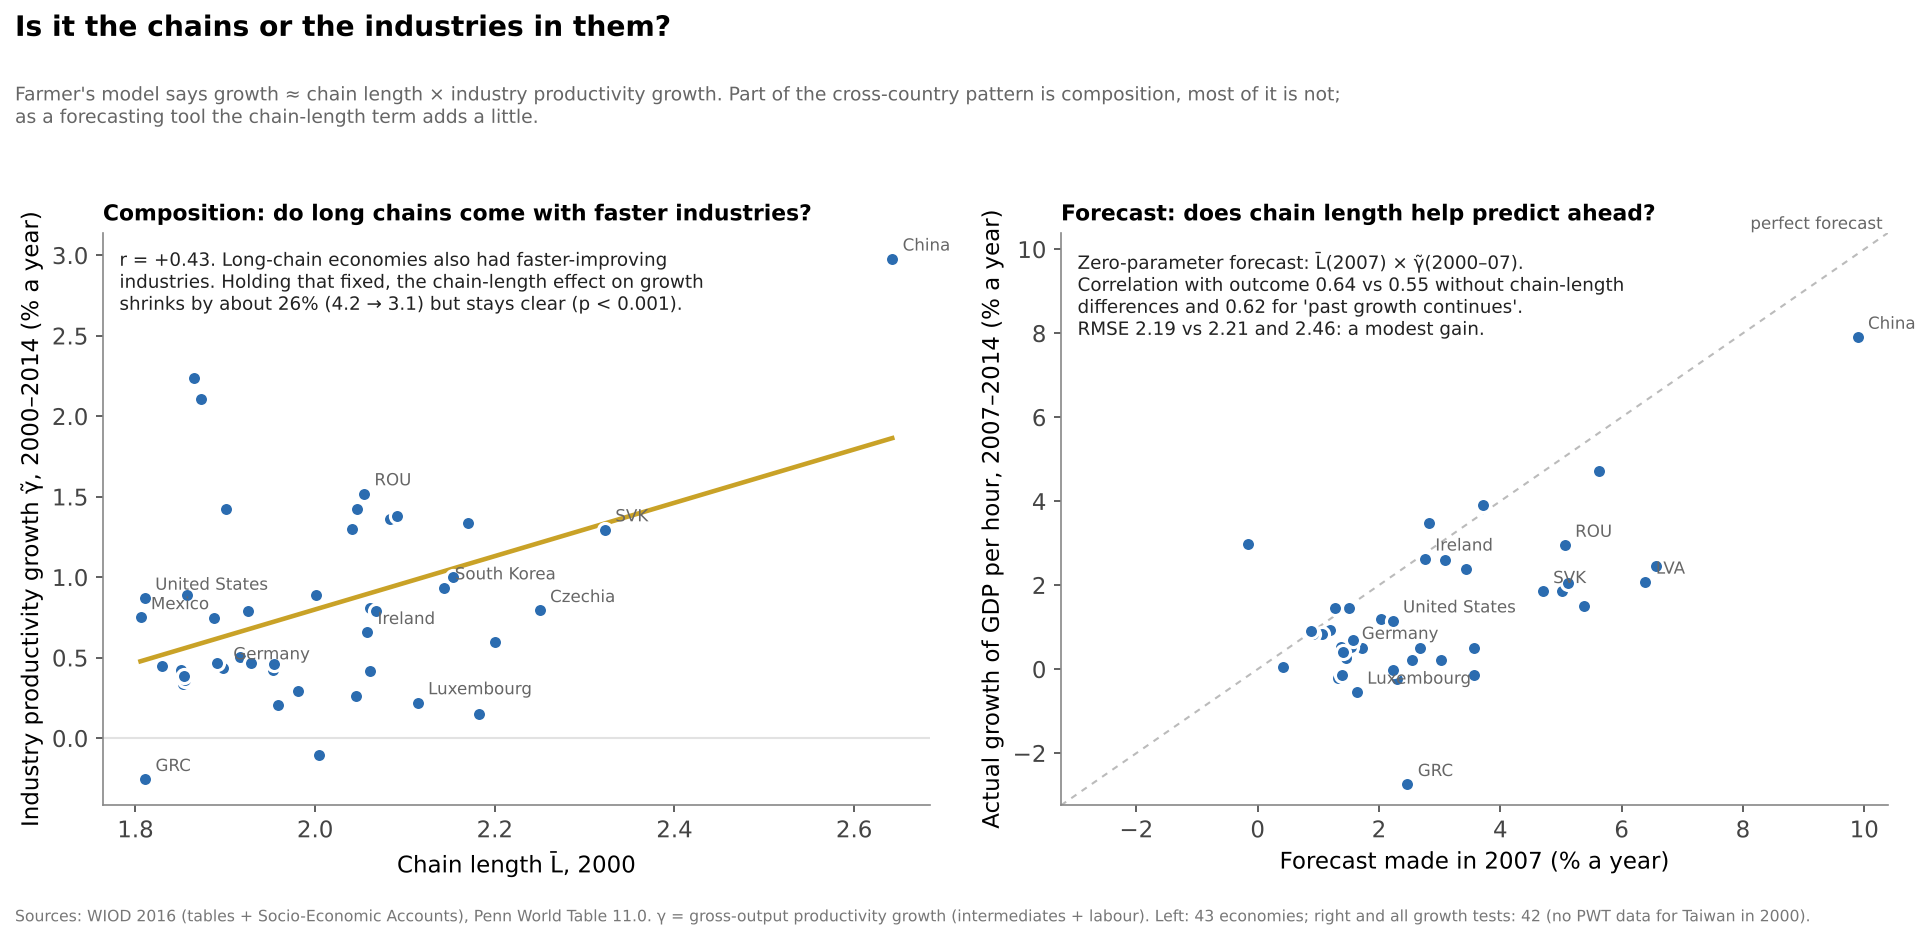
\includegraphics[width=\textwidth]{13_chains_or_links.png}
\caption{Left: chain length and industry productivity growth across economies.
Right: zero-parameter forecast of 2007--2014 growth.}
\label{fig:chains}
\end{figure}

\subsection{Within countries: no detectable effect}

The cross-country pattern does not carry over to changes within a country. With
country fixed effects, the WIOD estimate is imprecise ($p=\WithinWiodP$) and the
ICIO estimate is close to zero ($p=\WithinIcioP$). A country whose chains
lengthen over three years does not grow detectably faster over the next three
(WIOD $p=\DeepWiodP$; ICIO $p=\DeepIcioP$). An earlier version of our own study
reported such a ``deepening'' effect with the domestic measure on ICIO; it
reappears in that sample ($p=\DeepDomIcioP$) but does not replicate on WIOD
($p=\DeepDomWiodP$). Pooled non-overlapping windows, which compare countries
rather than track them, confirm the cross-country pattern (WIOD
\PooledWiodBeta{}, \PooledWiodP; ICIO \PooledIcioBeta{}, \PooledIcioP).

\subsection{Do prices fall faster at the end of long chains?}

The mechanism requires that industries with longer chains see their prices fall
faster relative to wages. Across \PriceN{} WIOD industries, comparing industries
within the same country, they do: one standard deviation of the multiplier goes
with \PriceBeta{} percentage points a year (\PriceP; Figure~\ref{fig:prices},
left). Comparing the \emph{same} industry across countries, the relation
disappears (\PriceIndBeta{}, $p=\PriceIndP$; right). The first result fits the
mechanism, but it also fits a simpler story in which long-chain industries such
as manufacturing improve faster on their own; the second suggests that, within
an industry, how long its chain happens to be in a given country does not change
how fast its price falls.

\begin{figure}[t]
\centering
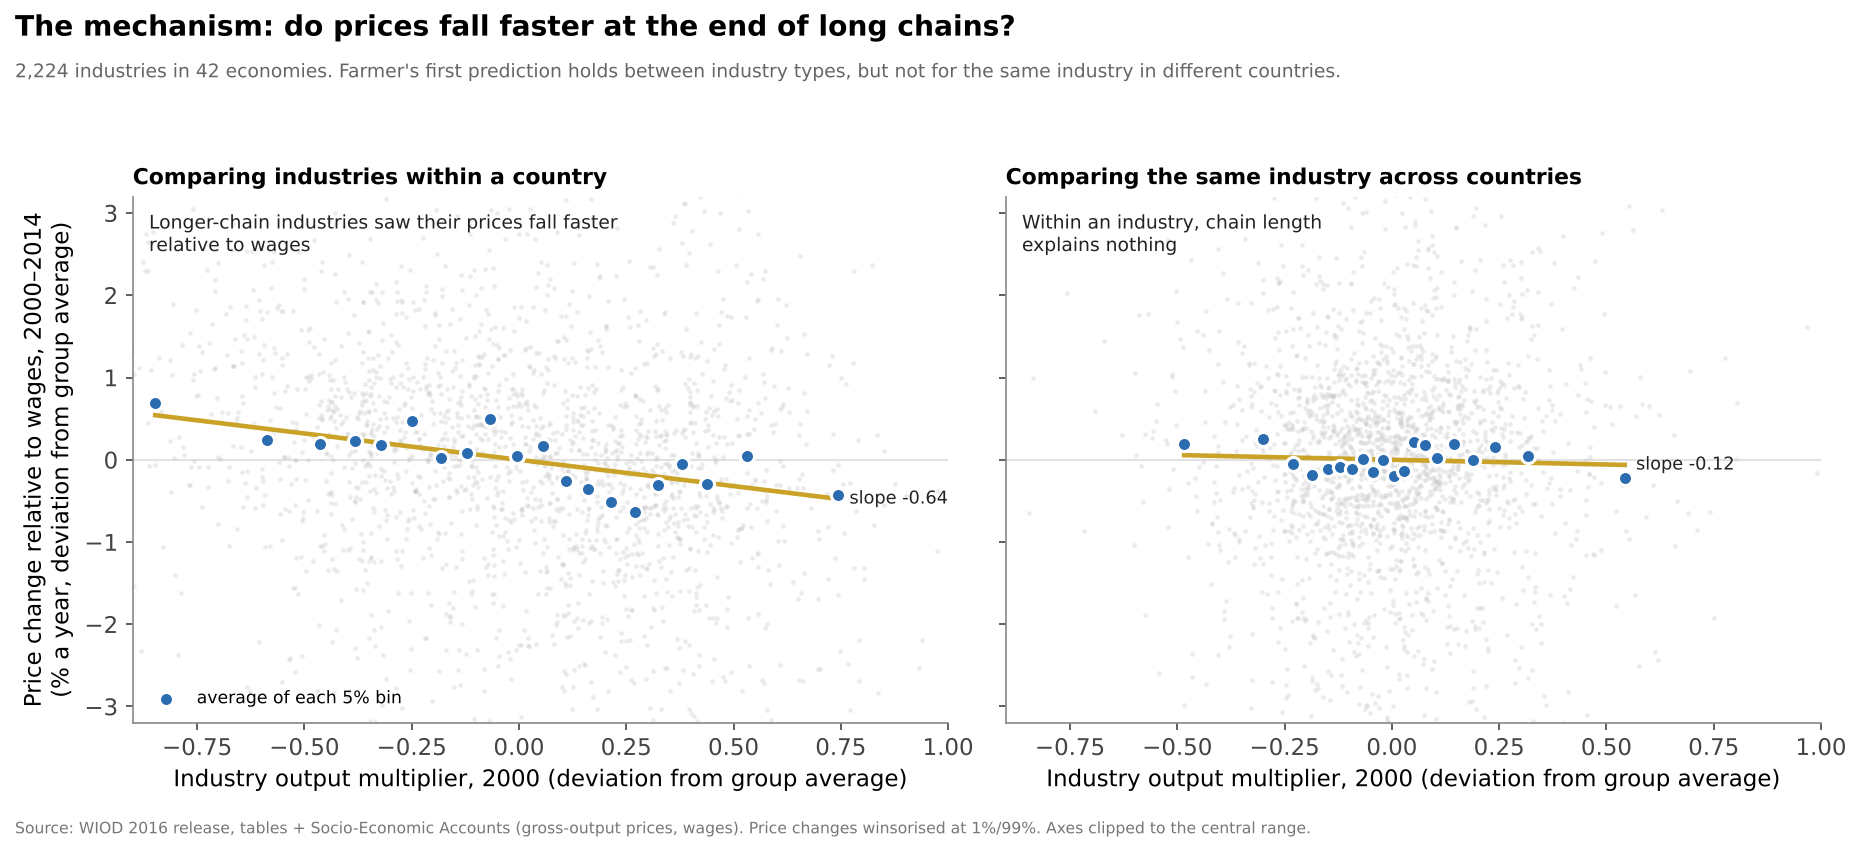
\includegraphics[width=\textwidth]{12_price_mechanism.png}
\caption{Industry price changes relative to wages, 2000--2014, against the 2000
output multiplier, after removing country means (left) and country and industry
means (right). Blue points are averages of 5\% bins.}
\label{fig:prices}
\end{figure}

\section{Discussion: what have we learned?}\label{sec:discussion}

The production-network view of growth passes a demanding replication. On a
different database and a later period, using the outcome the original authors
chose, the cross-country link between chain length and productivity growth is
about as strong as originally reported, and it survives the controls a sceptic
would try first. That is not common for a single-correlation result in
cross-country growth research.

What the evidence supports is a regularity \emph{between} economies, not yet a
lever \emph{within} them. Three readings are consistent with what we find.
\begin{enumerate}
\item \textbf{Amplification is real but slow.} Chain length moves slowly and the
effect works over decades; ten to fifteen years of annual tables leave too
little within-country variation to detect it. Longer panels (the 2025 OECD
edition covers 1995--2022) are the natural next test.
\item \textbf{Chain length marks a type of economy.} Long chains go with
manufacturing, integration in global supply chains and catch-up. Part of the
pattern is composition (\AmpShare\%), and in the ICIO sample long chains cannot be
separated from imported inputs. On this reading, chain length is a good summary
statistic of a growth-friendly structure rather than its cause.
\item \textbf{The mechanism operates across industry types.} The price evidence
fits a world in which long-chain industries are the ones where technology
improves fastest, which would make the network a channel for diffusion rather
than an independent multiplier.
\end{enumerate}

For policy, the safe conclusion is modest. Countries that participate in long
production chains have tended to grow faster, and measuring chains on the
domestic table alone misses the point for small open economies. Whether
deliberately lengthening chains would raise growth is not something these data
can settle.

\section{Limitations}\label{sec:limits}

\begin{itemize}
\item \textbf{Small samples.} 30--43 countries; we use resampling inference and
report all estimates, but power is limited, especially in subsamples.
\item \textbf{Many specifications.} The main grid has \NEstimates{} estimates. We
present them all rather than choosing; the pattern is consistent in sign across
the cross-country rows, but individual $p$-values should be read with that in
mind.
\item \textbf{Nominal tables.} Input coefficients come from tables at current
prices, so chain length can move with relative prices (for example, oil).
\item \textbf{Aggregation.} With 45--56 industries, part of every chain is hidden
inside industries; chain lengths are comparable across countries only at a
common classification.
\item \textbf{Productivity measurement.} $\gamma$ uses persons engaged rather than
hours (hours are missing for China), the main variant omits capital, and missing
industries are imputed.
\item \textbf{Multinational accounting.} Profit shifting inflates measured output
in economies such as Ireland and Luxembourg.
\item \textbf{An error we corrected.} A first run of our tests measured the
catch-up control in national currency units, which made it meaningless across
countries. Correcting it (to PPP levels) reduced the cross-country coefficients by
about a third and changed one conclusion (the convergers' role). All results here
use the corrected control.
\end{itemize}

\section{Reproducibility}\label{sec:repro}

All code, intermediate results and figures are in the public repository
\url{https://github.com/therestofeden/illuminations}, folder
\texttt{economics/trophic-structure}. Every number in this paper is generated
from the result files by \texttt{paper/make\_numbers.py}. The full pipeline, from
downloading the raw data to the figures, reproduces byte-for-byte from a clean
copy with a fixed random seed.

\section*{Acknowledgements and disclosure}
The analysis, code and first draft of this paper were produced with the
assistance of an AI model (Claude, Anthropic), under the author's direction; the
author is responsible for all content and errors. The author has no financial
interests related to this work.

\bibliographystyle{plainnat}
\bibliography{refs}

\appendix
\section{All estimates}\label{app:all}
{\footnotesize
\setlength{\tabcolsep}{4pt}
\begin{longtable}{ll>{\raggedright\arraybackslash}p{4.6cm}lrrrr}
\toprule
Test & Data & Specification & Measure & $\beta$/SD & $p$ (an.) & $p$ (res.) & $n$ \\
\midrule
\endhead
A & ICIO & 2011$\to$2019 raw & Farmer & +1.24 & $<0.001$ & 0.002 & 30 \\
A & ICIO & 2011$\to$2019 + catch-up & Farmer & +0.84 & 0.003 & 0.004 & 30 \\
A & ICIO & 2011$\to$2019 + catch-up + import intensity & Farmer & +0.85 & 0.082 & 0.115 & 30 \\
A & ICIO & 2011$\to$2019 + catch-up, per-capita growth & Farmer & +0.65 & 0.014 & 0.012 & 30 \\
A & ICIO & 2011$\to$2019 + catch-up + import int., per-capita & Farmer & +0.36 & 0.534 & 0.578 & 30 \\
A & ICIO & 2011$\to$2019 + catch-up, excl. fast convergers & Farmer & +0.53 & 0.049 & 0.068 & 26 \\
A & ICIO & 2011$\to$2019 + catch-up & v1 dom. & +0.16 & 0.746 & 0.770 & 30 \\
A & ICIO & 2011$\to$2023 raw & Farmer & +1.15 & $<0.001$ & 0.001 & 30 \\
A & ICIO & 2011$\to$2023 + catch-up & Farmer & +0.83 & 0.003 & 0.003 & 30 \\
A & ICIO & 2011$\to$2023 + catch-up + import intensity & Farmer & +0.81 & 0.106 & 0.157 & 30 \\
A & ICIO & 2011$\to$2023 + catch-up, per-capita growth & Farmer & +0.56 & 0.022 & 0.024 & 30 \\
A & ICIO & 2011$\to$2023 + catch-up + import int., per-capita & Farmer & +0.30 & 0.566 & 0.611 & 30 \\
A & ICIO & 2011$\to$2023 + catch-up, excl. fast convergers & Farmer & +0.62 & 0.040 & 0.053 & 26 \\
A & ICIO & 2011$\to$2023 + catch-up & v1 dom. & +0.29 & 0.539 & 0.592 & 30 \\
A & WIOD & 2000$\to$2014 raw & Farmer & +1.12 & $<0.001$ & $<0.001$ & 42 \\
A & WIOD & 2000$\to$2014 + catch-up & Farmer & +0.70 & $<0.001$ & $<0.001$ & 42 \\
A & WIOD & 2000$\to$2014 + catch-up + import intensity & Farmer & +0.77 & $<0.001$ & 0.001 & 42 \\
A & WIOD & 2000$\to$2014 + catch-up, per-capita growth & Farmer & +0.72 & $<0.001$ & $<0.001$ & 42 \\
A & WIOD & 2000$\to$2014 + catch-up + import int., per-capita & Farmer & +0.77 & $<0.001$ & 0.001 & 42 \\
A & WIOD & 2000$\to$2014 + catch-up, excl. fast convergers & Farmer & +0.62 & 0.074 & 0.086 & 28 \\
A & WIOD & 2000$\to$2014 + catch-up & v1 dom. & +0.50 & 0.020 & 0.037 & 42 \\
A & WIOD & 2000$\to$2019 raw & Farmer & +1.06 & $<0.001$ & 0.001 & 43 \\
A & WIOD & 2000$\to$2019 + catch-up & Farmer & +0.69 & $<0.001$ & $<0.001$ & 43 \\
A & WIOD & 2000$\to$2019 + catch-up + import intensity & Farmer & +0.76 & $<0.001$ & $<0.001$ & 43 \\
A & WIOD & 2000$\to$2019 + catch-up, per-capita growth & Farmer & +0.69 & $<0.001$ & $<0.001$ & 43 \\
A & WIOD & 2000$\to$2019 + catch-up + import int., per-capita & Farmer & +0.65 & $<0.001$ & 0.003 & 43 \\
A & WIOD & 2000$\to$2019 + catch-up, excl. fast convergers & Farmer & +0.69 & 0.052 & 0.058 & 29 \\
A & WIOD & 2000$\to$2019 + catch-up & v1 dom. & +0.47 & 0.027 & 0.048 & 43 \\
A & WIOD & 2000$\to$2023 raw & Farmer & +1.01 & $<0.001$ & $<0.001$ & 43 \\
A & WIOD & 2000$\to$2023 + catch-up & Farmer & +0.69 & $<0.001$ & $<0.001$ & 43 \\
A & WIOD & 2000$\to$2023 + catch-up + import intensity & Farmer & +0.72 & $<0.001$ & $<0.001$ & 43 \\
A & WIOD & 2000$\to$2023 + catch-up, per-capita growth & Farmer & +0.60 & $<0.001$ & $<0.001$ & 43 \\
A & WIOD & 2000$\to$2023 + catch-up + import int., per-capita & Farmer & +0.55 & $<0.001$ & 0.005 & 43 \\
A & WIOD & 2000$\to$2023 + catch-up, excl. fast convergers & Farmer & +0.70 & 0.042 & 0.049 & 29 \\
A & WIOD & 2000$\to$2023 + catch-up & v1 dom. & +0.42 & 0.047 & 0.075 & 43 \\
B & WIOD & pooled + period FE + catch-up & Farmer & +0.81 & $<0.001$ & 0.002 & 129 \\
B & WIOD & within-country (country + period FE) & Farmer & +0.74 & 0.313 & 0.243 & 129 \\
B & WIOD & pooled + period FE + catch-up & v1 dom. & +0.47 & 0.055 & 0.245 & 129 \\
B & WIOD & within-country (country + period FE) & v1 dom. & +0.81 & 0.209 & 0.145 & 129 \\
B & ICIO & pooled + period FE + catch-up & Farmer & +0.88 & 0.002 & 0.012 & 58 \\
B & ICIO & within-country (country + period FE) & Farmer & +0.12 & 0.847 & 0.810 & 58 \\
B & ICIO & pooled + period FE + catch-up & v1 dom. & +0.45 & 0.254 & 0.541 & 58 \\
B & ICIO & within-country (country + period FE) & v1 dom. & +0.62 & 0.232 & 0.085 & 58 \\
C & WIOD & $\Delta$depth + catch-up + year FE & Farmer & +0.30 & 0.152 & 0.240 & 514 \\
C & WIOD & ... + past-3y growth (momentum) & Farmer & +0.27 & 0.079 & 0.125 & 514 \\
C & WIOD & $\Delta$depth + catch-up + year FE & v1 dom. & +0.12 & 0.600 & 0.794 & 514 \\
C & WIOD & ... + past-3y growth (momentum) & v1 dom. & +0.17 & 0.244 & 0.468 & 514 \\
C & ICIO & $\Delta$depth + catch-up + year FE & Farmer & +0.26 & 0.253 & 0.428 & 88 \\
C & ICIO & ... + past-3y growth (momentum) & Farmer & +0.16 & 0.460 & 0.519 & 88 \\
C & ICIO & $\Delta$depth + catch-up + year FE & v1 dom. & +0.65 & 0.018 & 0.111 & 88 \\
C & ICIO & ... + past-3y growth (momentum) & v1 dom. & +0.56 & 0.004 & 0.025 & 88 \\
D & WIOD & country FE & ind. $L$ glob. & -0.26 & $<0.001$ & $<0.001$ & 2224 \\
D & WIOD & country FE + industry FE (strict) & ind. $L$ glob. & -0.05 & 0.674 & 0.697 & 2224 \\
D & WIOD & country FE & ind. $L$ dom. & -0.15 & 0.035 & 0.041 & 2224 \\
D & WIOD & country FE + industry FE (strict) & ind. $L$ dom. & -0.01 & 0.934 & 0.933 & 2224 \\
\bottomrule
\end{longtable}

}

\end{document}
